\subsection{Possible Architectures and Related Diagrams}

\subsubsection{Proposed Sensor FOV Topology}
\noindent A ranging apparatus comprised of four ultrasonic sensors, one central LiDAR sensor, and optionally, a camera with spatial AI, should provide ample ability to FORWARD's object detection feature. Two wide FOV ultrasonic sensors face forward: one on each walker leg. Two face sideways, also mounted on the bottom half of the legs. The LiDAR sensor is mounted centrally so its beam detects straight-on obstacles. The camera is also mounted centrally. Finally, we angle these downward to allow for detection of obstacles present at the knee down height level. Additionally, a zero energy return from the ultrasonics or LiDAR could constitute a drop-off or ledge or divot. This will be elaborated upon in obstacle classification and identification.\\

\begin{figure}[H]
	\centering
	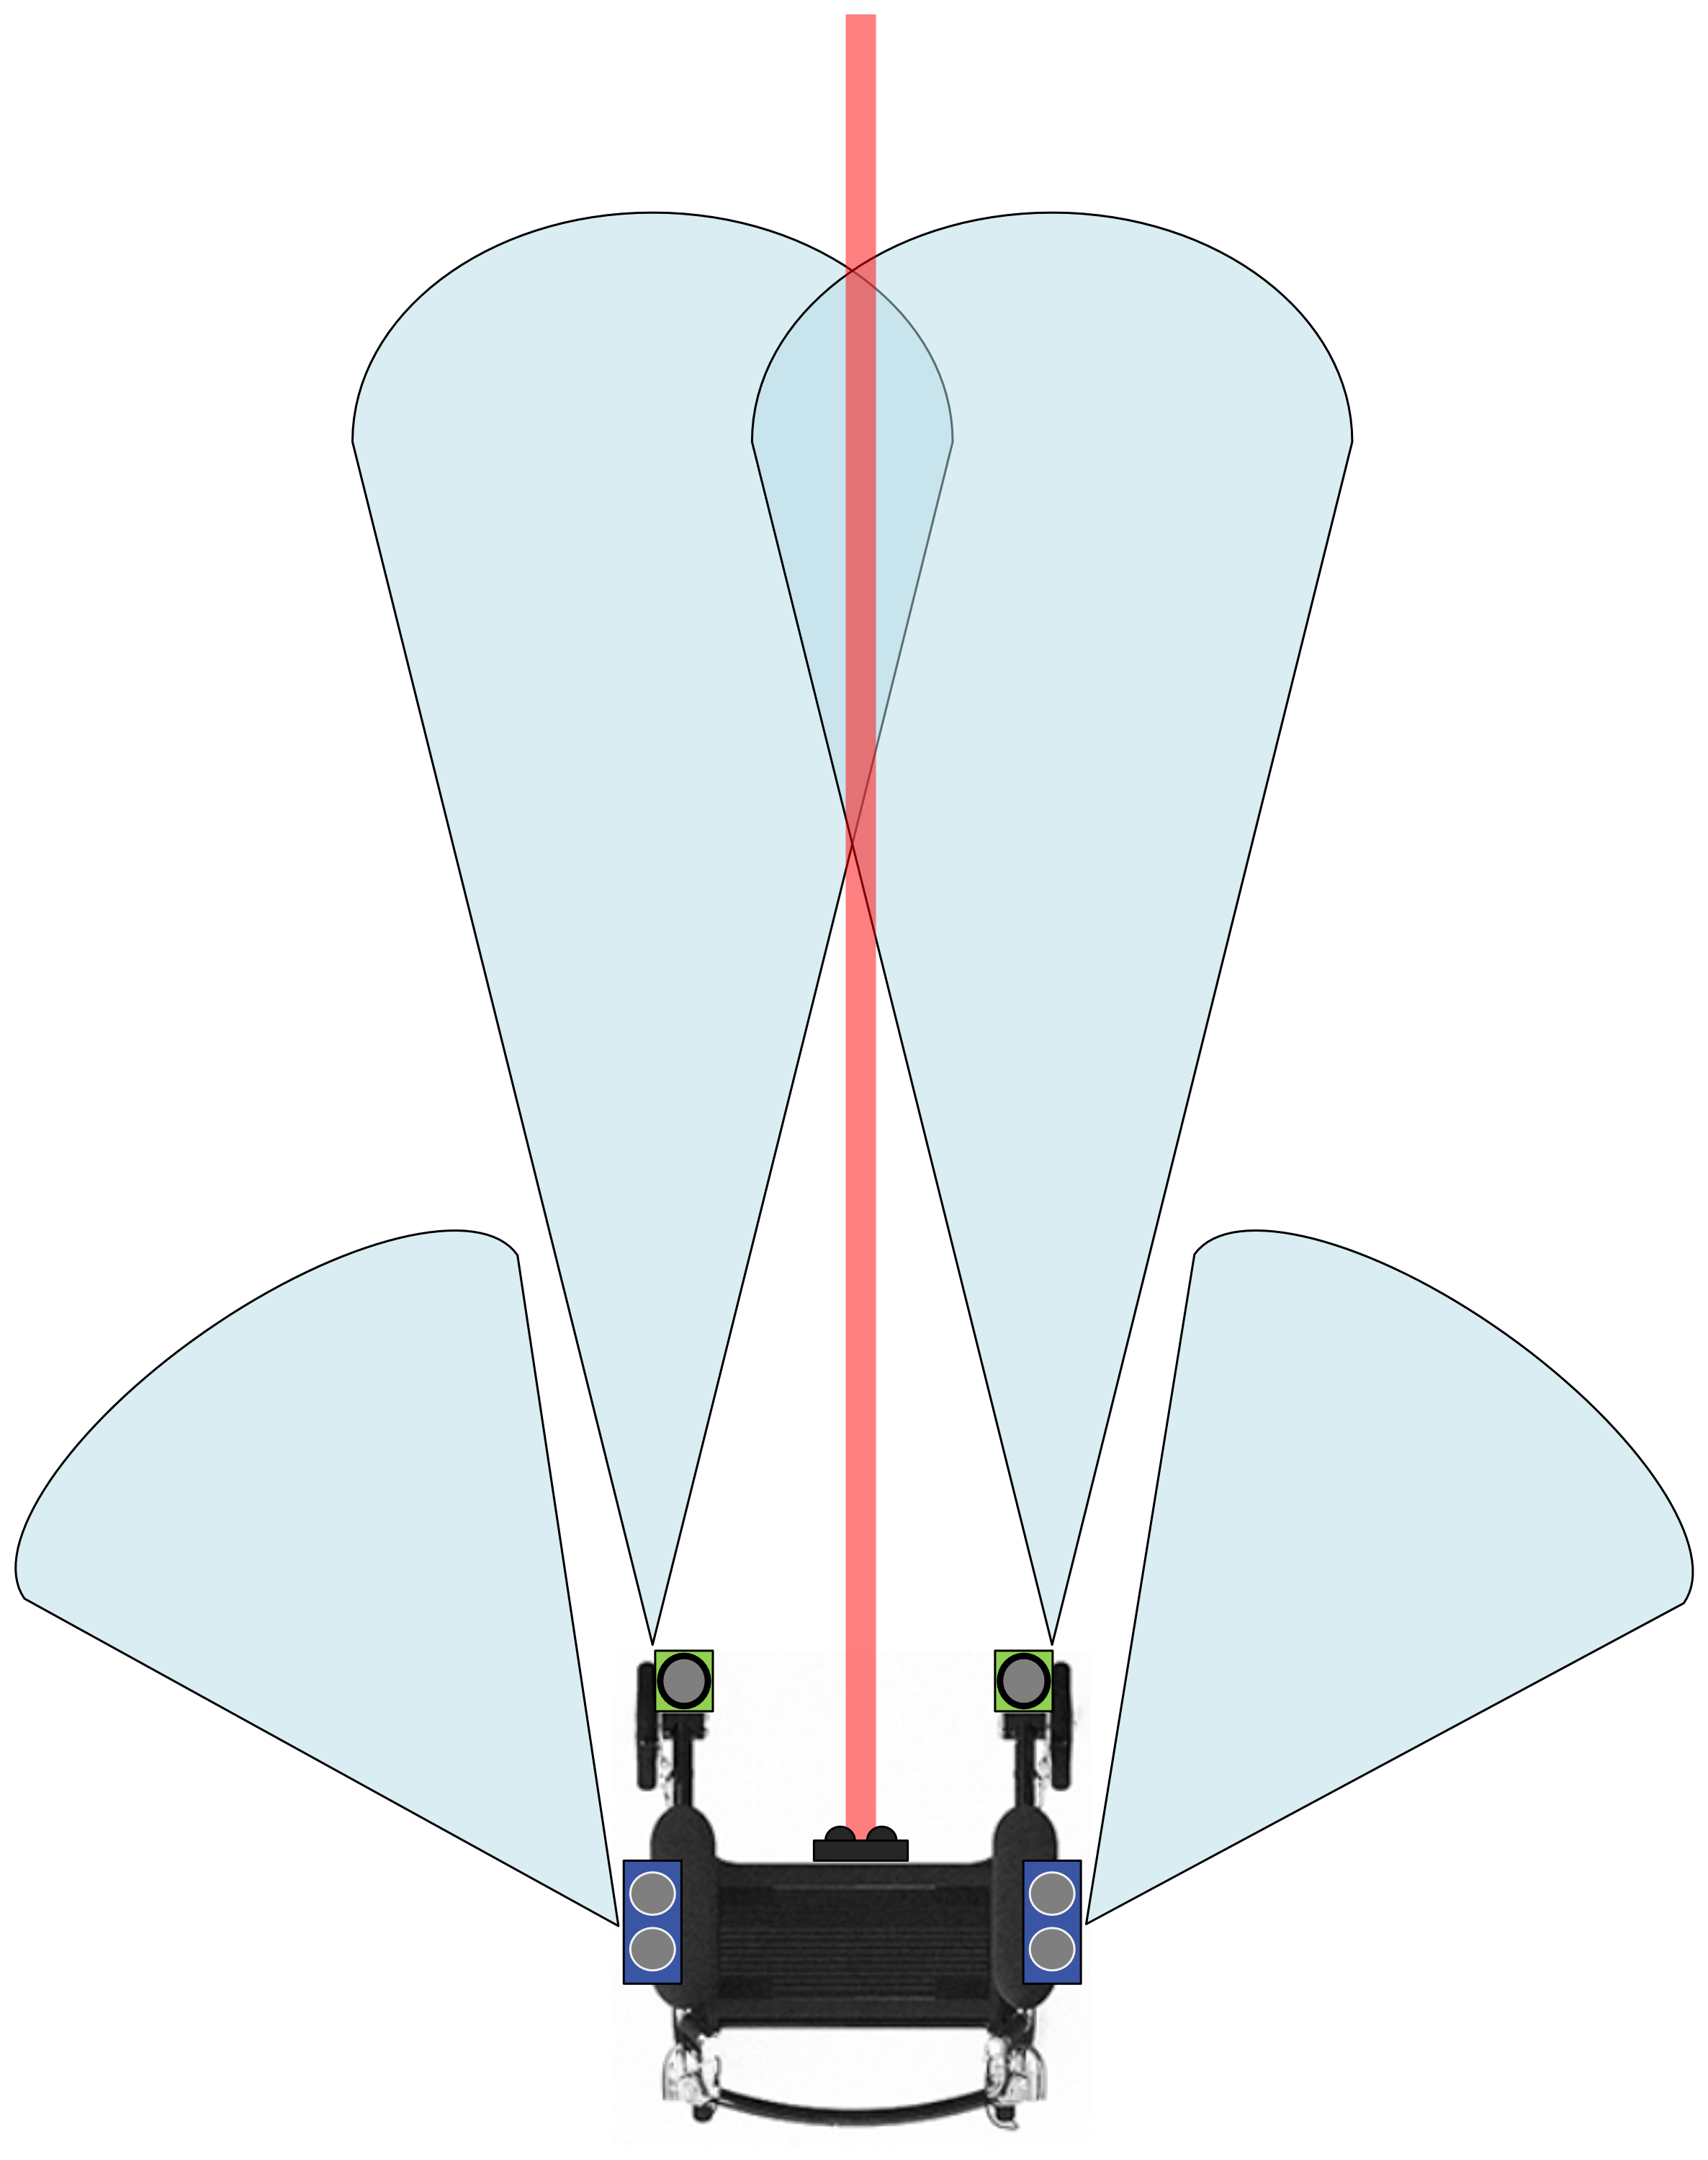
\includegraphics[angle=90,width=0.75\textwidth]{./Images/propose-sensorFOV.png}
	\caption{\label{fig:proposedsensorFOV}Proposed Sensor FOV (Range NOT to scale)}
\end{figure}

\noindent As mentioned in 2.2, the object detection data must work hand-in-hand with the identification and avoidance schemes. With identification, the range data is combined with any potential depth perception data generated by the camera. The closer the walker gets to the obstacle, the more urgently the system can respond. With avoidance, motor commands should be generated proportionately to the severity of the obstacle range-to-walker frame. Determining these specific plans of action is elaborated in later sections.\\

%\begin{figure}[h]
%	\centering
%	\includegraphics[width=0.7\textwidth]{./Images/FOVapparatus.png}
%	\caption{\label{fig:proposedFOVapparatus}Proposed Sensor Ranging Apparatus}
%\end{figure}
\subsubsection{Velocity and Position Solution}
\noindent With the addition of the IMU as indicated in section 3.3, FORWARD is able to resolve its relative velocity and position based on a starting point by twice integrating the accelerometer data output. By tracking these updates, FORWARD can be more self-aware of its current traveling state. Not only is the IMU useful for tilt detection (identifying incline and decline), but it can also be used to verify and validate the range data output by the LiDAR and sonar sensors. For example, the software can have some condition where, if the range decreases under a predetermined threshold of danger, then the IMU data can reset and begin tracking position and velocity, with that initial point as the origin of the reference frame. This can allow for very precise geometric abstracted data visualization of the free space ahead and the trajectory of the walker.\\

\subsubsection{Kalman Filter}
\noindent As part of the project stretch requirement for depth perception using an upgraded camera, implementation of a typical sensor fusion algorithm will help to predict the walker's trajectory and provide counteractive insight to the guidance system. Implementation of a Kalman filter estimator would not be beneficial for the fusion of the LiDAR and Sonar data, because the delta between these should be small, and thus, would not provide any helpful insight to FORWARD. However, if obtaining a second range solution from AI depth perception, this data could be fused to choose how much credence is given to either the standard range solution or the computer vision. Essentially, this functionality would be able to minimize measurement noise originating from the information loss of the sensors, and to maximize the overall precision of obstacle avoidance.\\

% matthew
\subsubsection{Typical CV camera setup}

% morgan
\subsubsection{Typical steering motor control wiring}